\documentclass{article}
\usepackage[utf8]{inputenc}
\usepackage[polish]{babel}
\usepackage{polski}
\usepackage{enumerate}
\usepackage{natbib}
\usepackage{graphicx}
\usepackage{geometry}
\usepackage{float}
%\usepackage{hyperref}
\usepackage{url}

\newgeometry{tmargin=2.3cm, bmargin=2.5cm, lmargin=2.5cm, rmargin=2.5cm}

\makeatletter
\newcommand{\linia}{\rule{\linewidth}{0.4mm}}
\renewcommand{\maketitle}{\begin{titlepage}
    \vspace*{1cm}
    \begin{center}
    Politechnika Wrocławska\\
    AiR ARR\\
 Projekt zespołowy
    \end{center}
      \vspace{3cm}
    \begin{center}

     \LARGE \textsc {\@title}
         \end{center}
     \vspace{1cm}

    \begin{center}
    \textit{ Autorzy:}\\
   \textit{\@author}
     \end{center}
      \vspace{1cm}

     \begin{center}

    Prowadzący:
  dr inż. Krzysztof Arent
    \end{center}

    \vspace*{\stretch{6}}
    \begin{center}
    \@date
    \end{center}
  \end{titlepage}
}
\makeatother
\author{Beata Berajter\\
Dawid Brząkała\\
Dorota Gidel\\
Katarzyna Wądrzyk\\
Ada Weiss\\
Małgorzata Witka-Jeżewska\\
 }
\title{SensGlove}

\begin{document}

\maketitle
\newpage
\tableofcontents
\newpage




%%%%%%%%%%%%%%%%%%%%%%%%%
% Ogólnie:
% zrealizowane części projektu
% sposób ich zrealizowania
% niezrealizowane
% dlaczego nie
%
%
%
% Pozmieniałam tytuły dla punktu 2.1, prosze zrobić coś w tym właśnie stylu, chyba że macie lepsze propozycje - można tak jak w punkcie 2.4 robić
%
%
% UWAGA! Tekst specyfkacji zostawiam po to, zebyscie nei musieli szukać! Należy go usunać albo chociaż zmienić na swoje potrzeby
%%%%%%%%%%%%%%%%%%%%%%%%%
\section{Opis stanowiska}
Stanowisko składa się z:
\begin{enumerate}
	\item rekawiczki z sensorami oraz okablowaniem
	\item 5 nakładek na palce oraz jednej na dłoń
	\item 8 sensorów biosygnałów
	\item 3 frotek
	\item przedwzmacniacza do biosygnałów
	\item płytki ze wzmacniaczami
	\item 2 baterii zasilających 9V
	\item płytki developerskiej STM32Discovery
	\item komputera z programami do akwizycji danych oraz do ich wizualizacji	
\end{enumerate}

\begin{figure}[H]
	\centering
	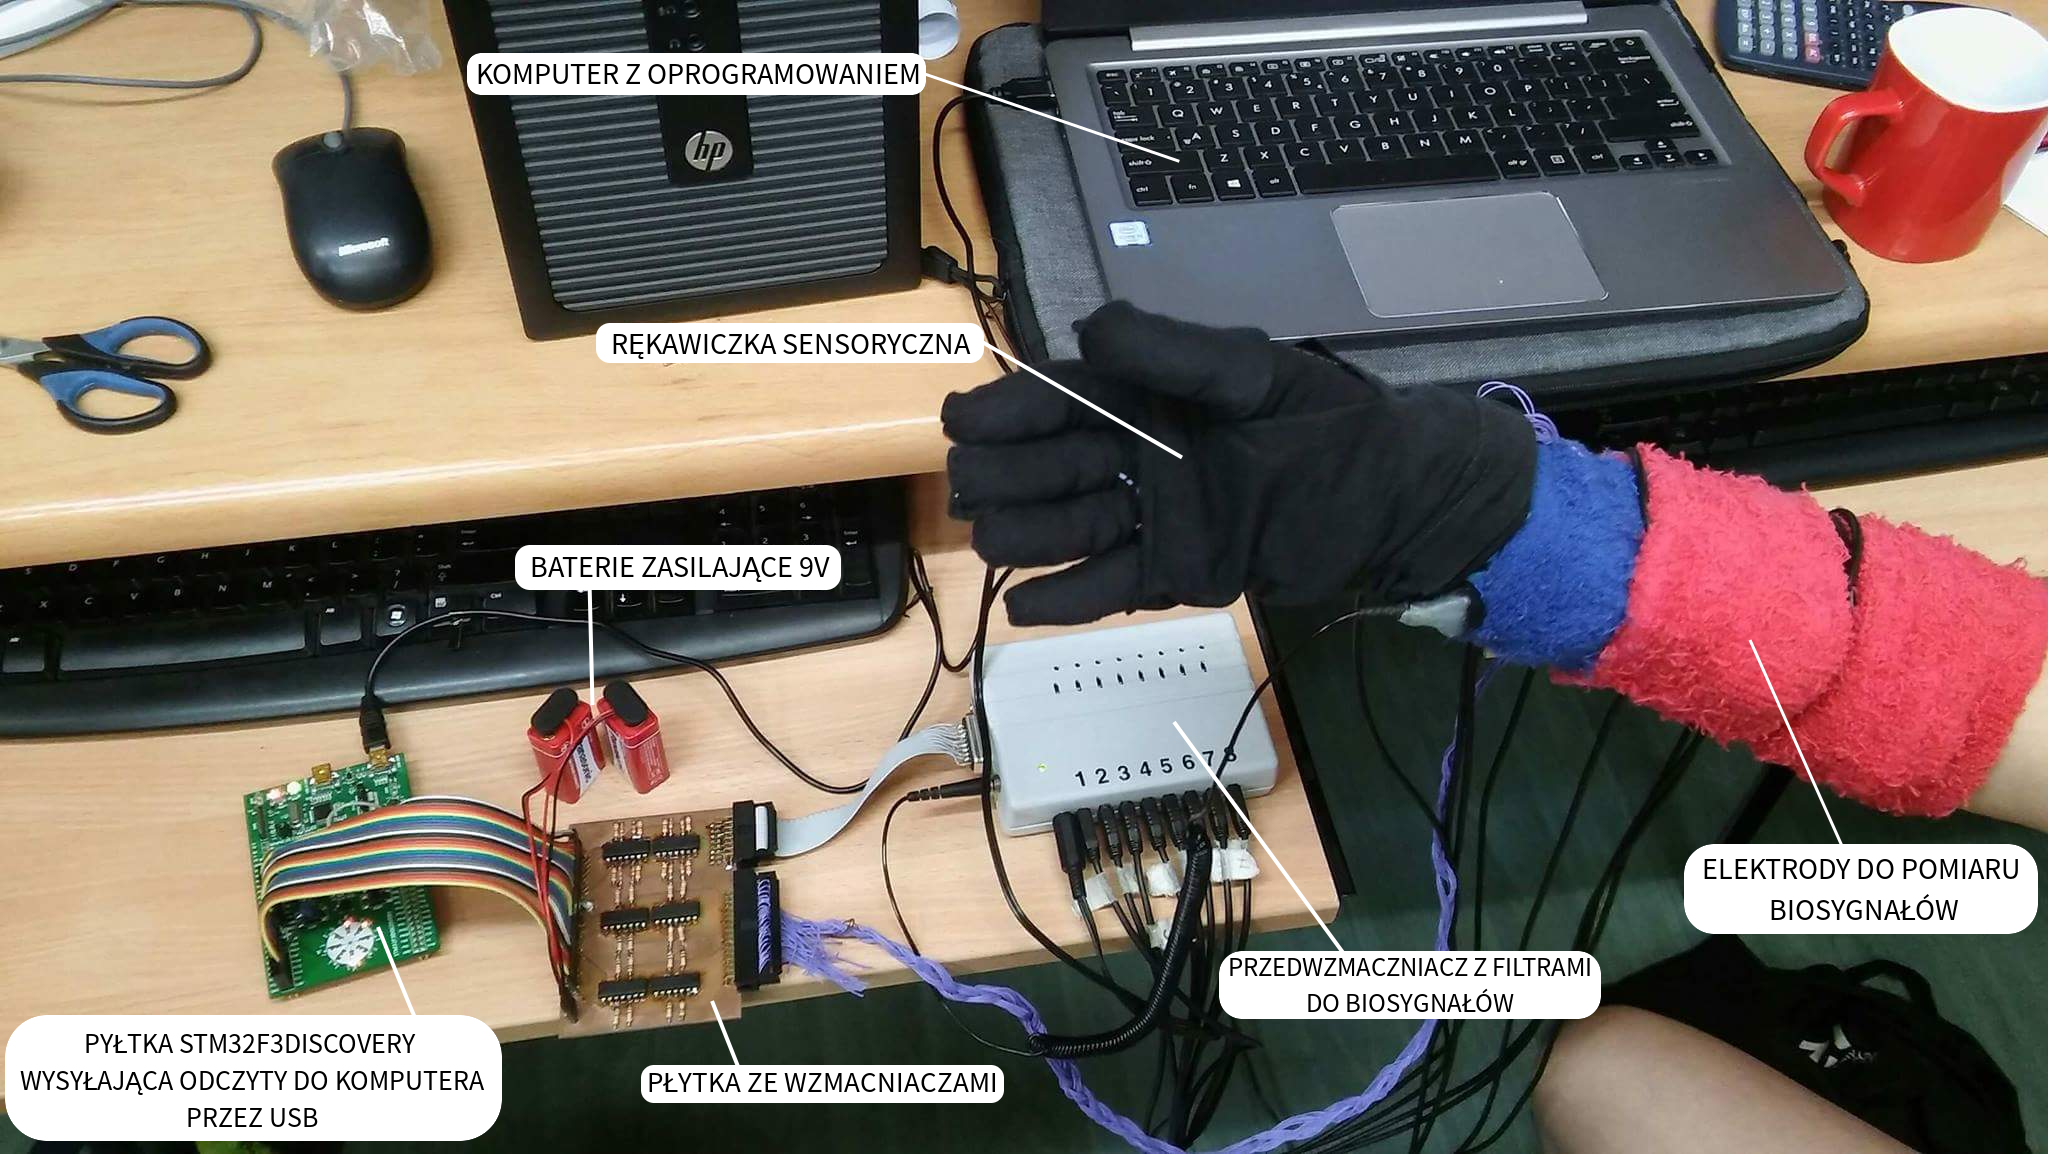
\includegraphics[width=16cm]{rekawiczka_opis_stanowiska.png}
	\caption{Opis komponentów stanowiska do pomiarów biosygnałów i sygnałów z rękawiczki sensorycznej}
	\label{rys:stanowisko}
\end{figure}

\begin{figure}[H]
	\centering
	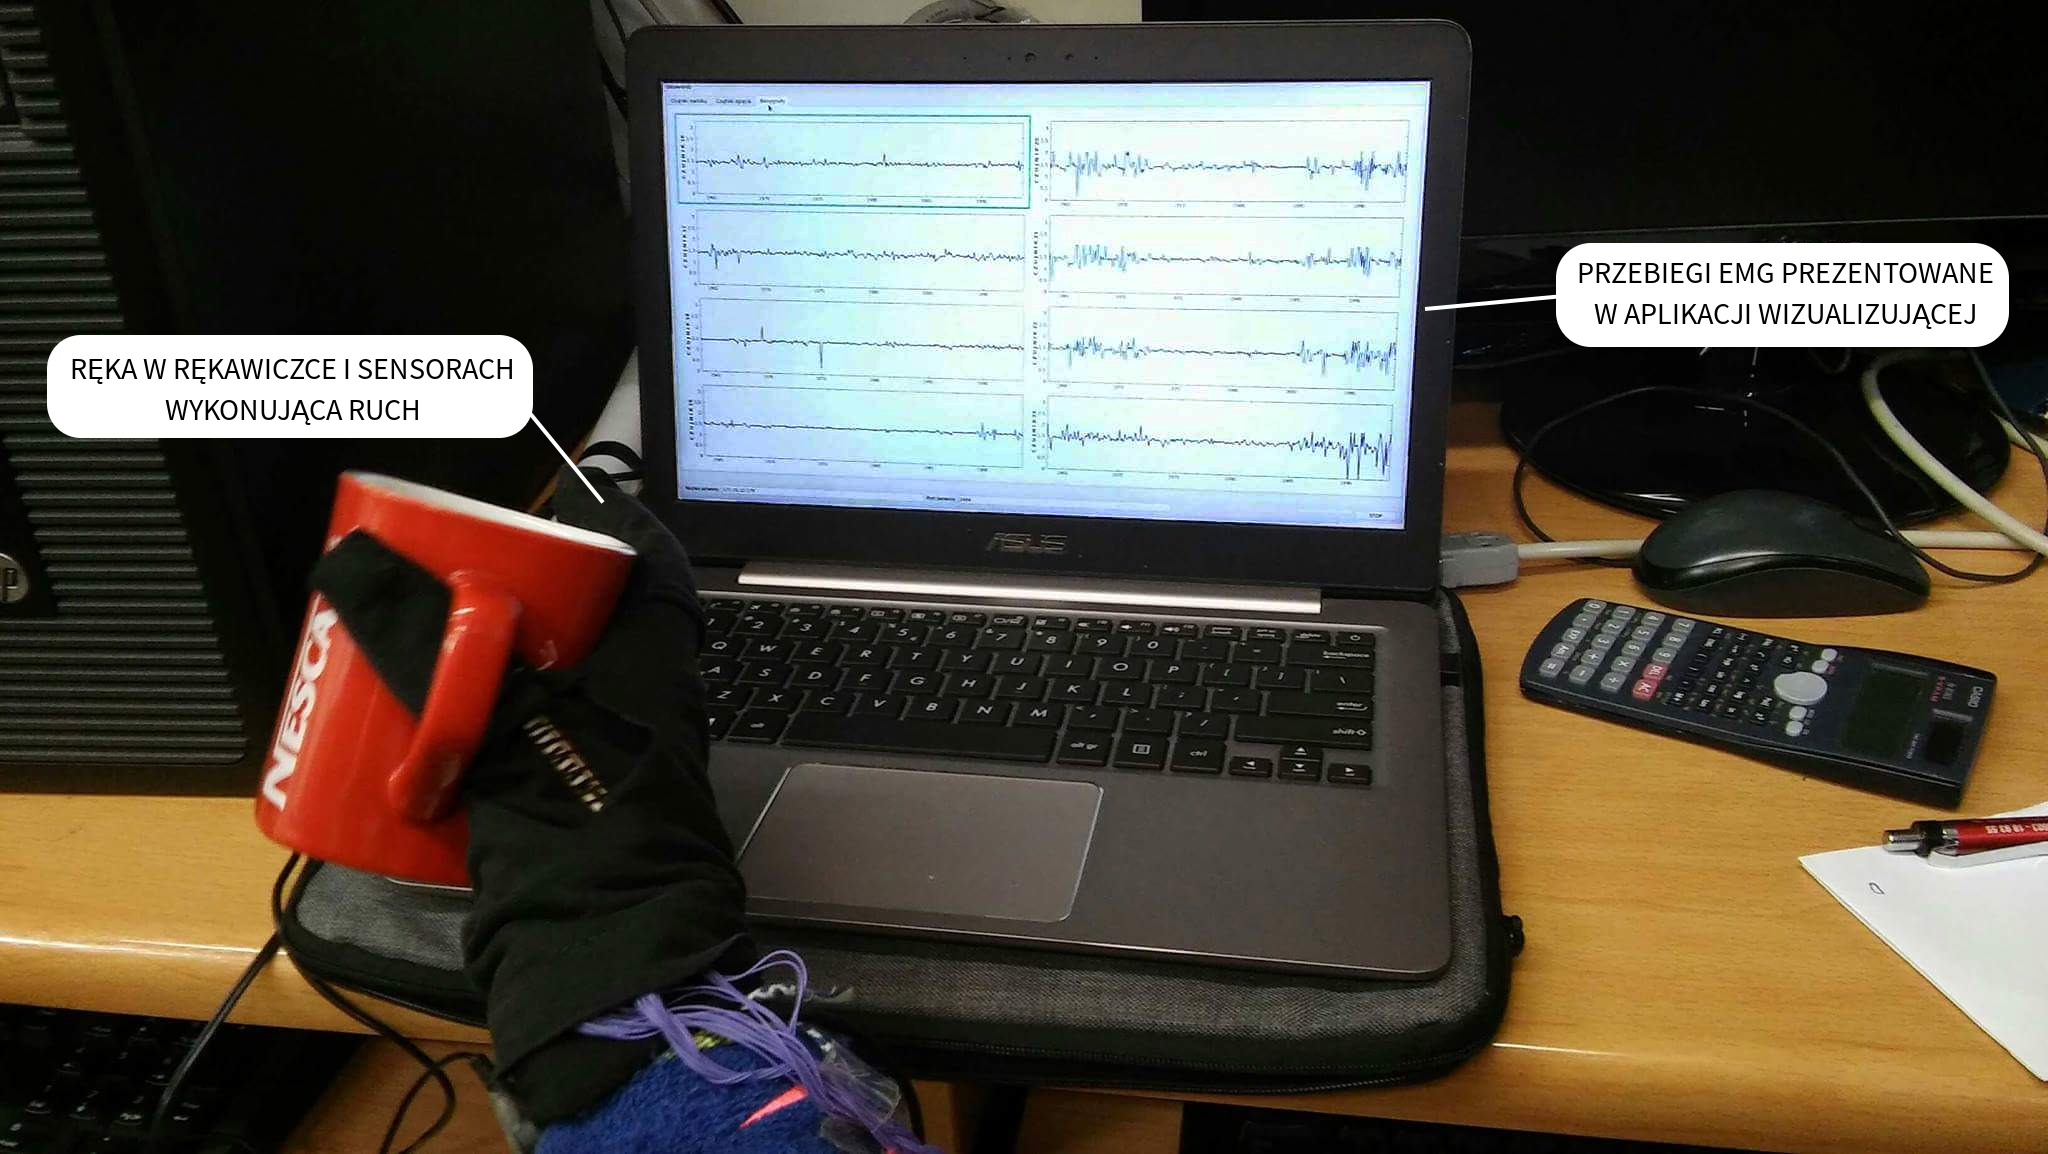
\includegraphics[width=16cm]{rekawiczka_aplikacja.png}
	\caption{Prezentacja odczytów zbieranych ze stanowiska do pomiarów}
	\label{rys:stanowisko}
\end{figure}

\subsection{Przygotowanie stanowiska}

\begin{enumerate}
  \item Należy nałożyć ostrożnie rękawiczkę na dłoń, uważając, by nie zginać nadmiernie czujników nacisku. Rękawiczka założona na rękę pozwala na możliwie swobodne poruszanie palcami.
	\item Podczas wykonywania ruchów czujniki oraz przewody nie haczą się o nic dzięki przyszyciu ich do rękawiczku, spleceniu oraz dzięki dołączonym kapturkom oraz dodatkowej bezpalcowej osłonie. Koniecznie należy je nałożyć na palce i dłoń szwami od strony czujników ugięcia w celu ich poprawnego działania.
	\item Sygnały z czujników prowadzone przez przewody są bezpośrednio podłączone do styków na wzmacniaczu dzięki przygotowanemu złączu przedstawionym na zdjęciu \ref{rys:koncowka}.
	\begin{figure}[H]
    \centering
    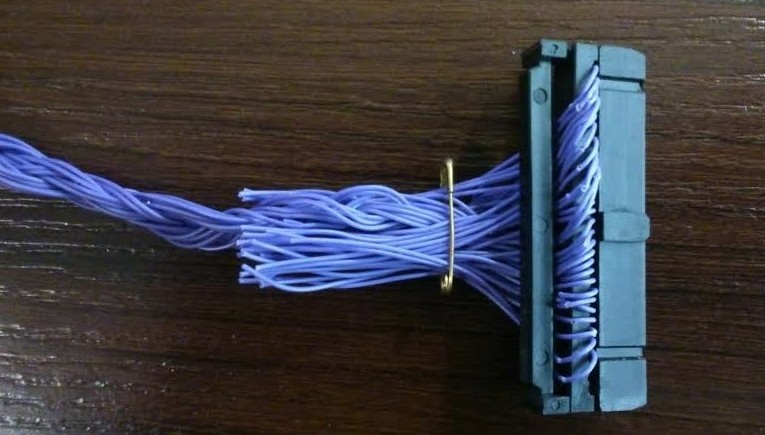
\includegraphics[width=9cm]{koncowka.jpg}
    \caption{Końcówka czujników pozwalająca na łatwe podłączenie do płytki ze wzmacniaczami}
    \label{rys:koncowka}
  \end{figure}
	
	\item Na przedramieniu osoby badanej należy umieścić sensory biosygnałów w sposób pokazany w instrukcji ''Stanowsiko badawcze do akwizycji biosygnałów'' autorstwa A. Wołczowskiego i J.S. Witkowskiego.
	\item Płytkę ze wzmacniaczami należy połączyć z płytką deweloperską Discovery, zasilaniem bateryjnym, wzmacniaczami biosygnałów oraz wtyczką z czujnikami nacisku oraz ugięcia w sposób pokazany na zdjęciu.
	\item Należy włączyć oba programy - do akwizycji danych oraz do ich wizualizacji. Dane z płytki Discovery płynnie przesyłane są poprzez przewód USB do komputera z włączonym programem do akwizycji danych.
	\item Poprzez obsługę programu do akwizycji danych pomiar rozpoczynany jest poprzez przyciśnięcie przycisku ''Start''.
	\item We włączonym programie od wizualizacji w odpowiednich zakładkach w czasie rzeczywistym można obserować przebieg sygnałów z czujników: nacisku, ugięcia i biosygnałów a także wizualizacje dłoni z czujnikami nacisku i ugiecia.
	\item Przy chwytaniu przedmiotów czujniki ugięcia działają sprawnie, o czym świadczy ugięcie palców na wirtualnej dłoni oraz wykresy z odczytami wartości rezystancji z czujników.
	\item Sensory nacisku na wewnętrznej części dłoni sprawnie odczytują siłę nacisku. Świadczy o tym zmiana koloru odpowiednich pól na wizualizowanej dłoni.
	\item Przy wybraniu odpowiednich zakładek widać na poszczególnych wykresach jak ruch wpływa na sygnały z czujników: ugięcia, nacisku i biosygnałów.
	\item Przy wciśnięciu przycisku ''Measurement'' w programie do akwizycji danych pojawia się pasek ładowania odmierzający 2 s. Po tym czasie pojawia się możliwość zapisu lub zignorowania danych.
	\item Po wybraniu ruchu i wpisaniu przykładowej nazwy użytkownika oraz przyciśnięciu przycisku ''Save'' wartości z pomiarów zostają poprawnie zapisane do odpowiedniego folderu. Przykładowy wynik tej operacji jest pokazany na rysunku \ref{rys:baza_folder}.
	
	\begin{figure}[H]
    \centering
    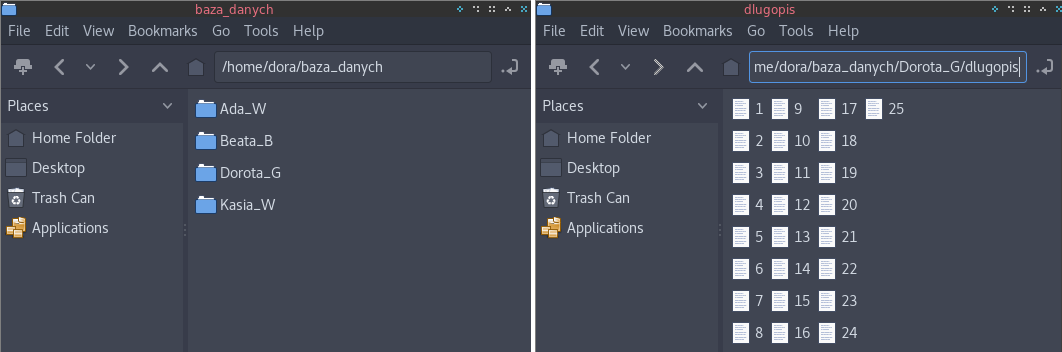
\includegraphics[width=15cm]{baza_folder.png}
    \caption{Poprawie utworzone foldery i pliki w bazie danych}
    \label{rys:baza_folder}
  \end{figure}
	
\end{enumerate}

%opis czynnnosci pozwalajacych polaczyc komponenty i wykonac pomiary
\section{Podsumowanie prac dla poszczególnych komponentów}

\subsection{Rękawiczka sensoryczna}
Osoby przydzielone do zadania: Dorota Gidel, Katarzyna Wądrzyk.
\subsubsection{Wykonanie rękawiczki}

Na rękawiczce wykonanej z poliestru przymocowano 9 czujników nacisku oraz 5 czujników ugięcia. Umiejscowienie czujników zostało przedstawione na rysunku \ref{rys:czujniki_numeracja}. Z powodu zniszczenia jednego czujnika nacisku został on odłączyony od rękawiczki. Istnieje jednak możliwość ponownego przymocowania go.\\
\begin{figure}[H]
    \centering
    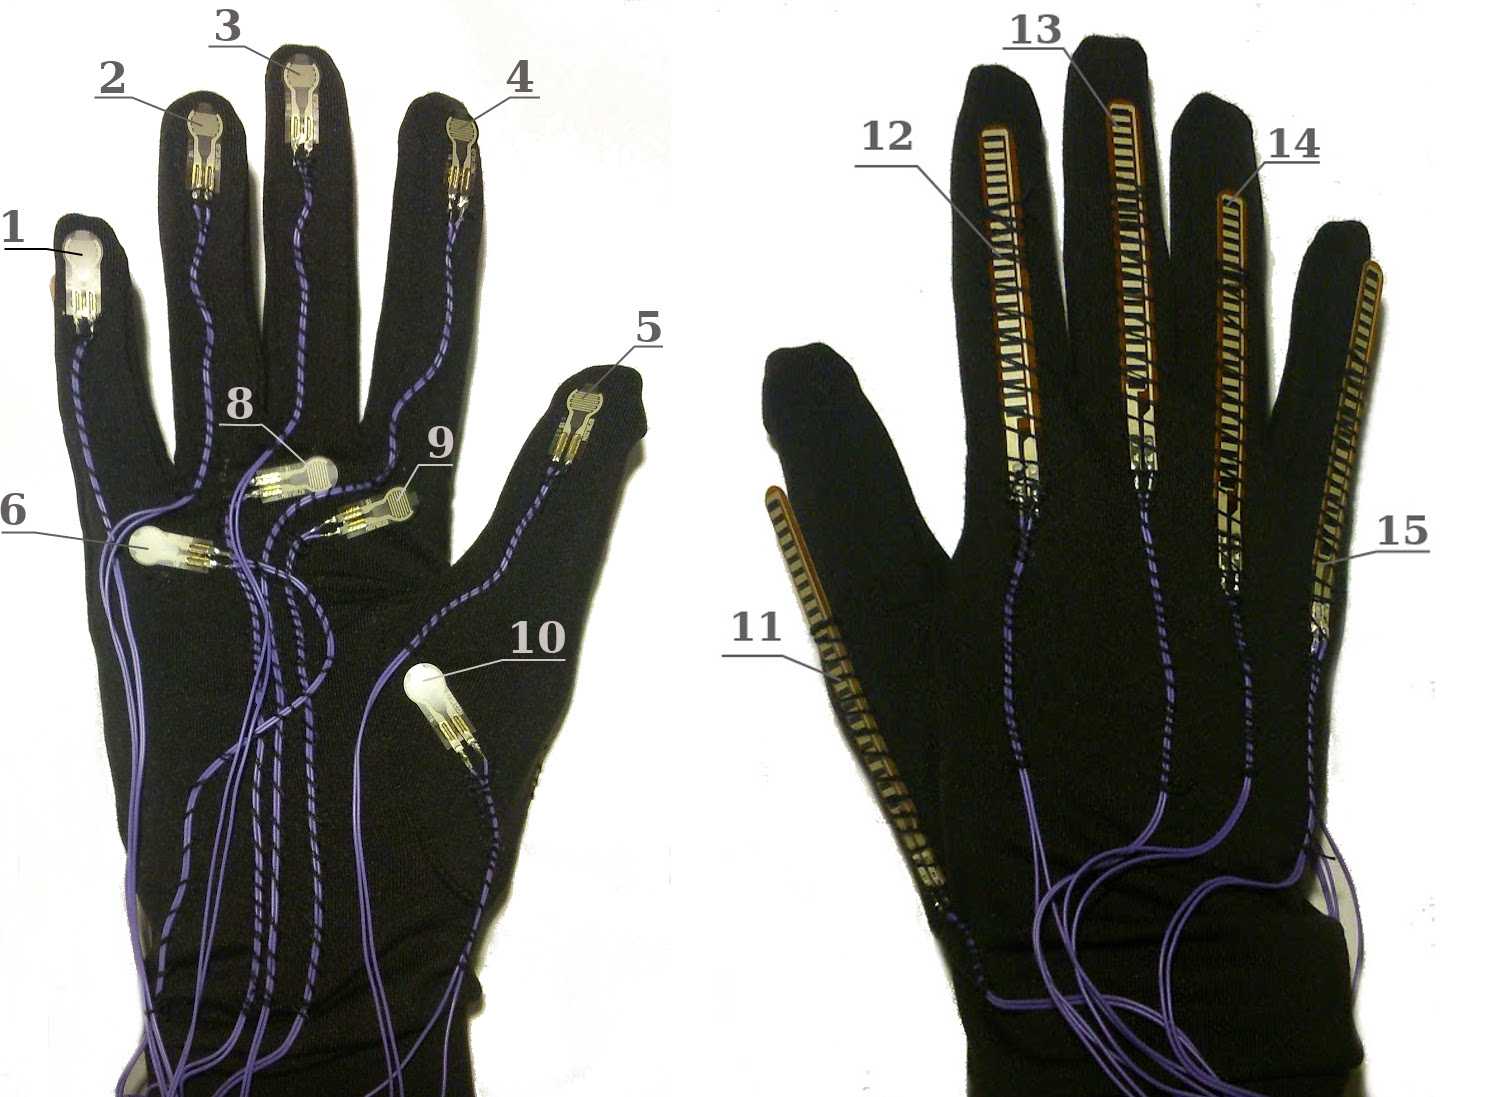
\includegraphics[width=14cm]{rekawiczka_umiejscowienie.jpg}
    \caption{Umiejscowienie i numeracja czujników na rękawiczce}
    \label{rys:czujniki_numeracja}
\end{figure}
Proces wykonania rękawiczki polegał na przylutowaniu przewodów do czujników, następnie przyklejeniu
punktowo klejem czujników w odpowiednich miejscach na rękawiczce oraz przyszycie przewodów do ręka-
wiczki, w przypadku czujników zgięcia przyszyto również część czujnika by mógł się poruszać.\\
Przyszycie przewodów pozwala na zachowanie porządku i sprzyja ruchom osoby używającej rękawiczkę a
przytwierdzenie klejem zapewnia trwałość. W celu zapobiegania uszkodzenia czujników (przede wszystkim
haczeniu) uszyte zostały ”kapturki” na palce. Dzięki nim sensory nacisku jak i także ugięcia są zabezpieczone
przed uszkodzeniami.\\
Na końcach przewodów odprowadzających sygnały z czujników zamontowane zostały żeńskie końce, które
umożliwiają proste podłączenie ich do płytki wzmacniającej. Przymocowane czujniki numerowane są w ko-
lejności przedstawioej na rysunku 1.\\

\subsubsection{Wprowadzone zmiany}
Planowowane było kupienie rękawiczki w rozmiarze S, ze względu na skład grupy, jednakże ostatecznie wybrano rozmiar M. Rękawiczka nadal dobrze dopasowuje się na dłoniach małych ale dodatkowo może z niej korzystać większe grono osób. Dzięki czemu do tworzenia bazy danych nie będzie potrzeby specjalnie wybierania i szukania osób o danym rozmiarze dłoni.\\
Zaletą większego rozmiaru jest też większa powierzchnia do mocowania czujników. Dużo łatwiej jest rozmieścić wszystkie sensory, po ich przymocowaniu nie ograniczają one ruchów w tak dużym stopniu jakby miało to miejsce przy rękawiczce o rozmiarze S.\\
Ze względu uszkodzenia się czujników, rękawiczka posiada 9 czujników nacisku. Jak widać na zdjęciu \ref{rys:czujniki_numeracja} czujnik 7 został pominięty, a czujnik 8 lekko przesunięty w lewą stronę by to zrekompensować. Jednakże dalej isnieje możliwość przymocowania brakującego czujnika 7.

\subsection{Interfejs sprzętowy}

Osoby przydzielone do zadania: Beata Berajter i Dawid Brząkała. \\
\subsection{Opis}
Interfejs sprzętowy składa się z płytki pcb wyposarzonej w wzmacniacze operacyjne, złącz czujników, złącza wyjść oraz zasilania. 
Drugim elementem interfejsu jest płytka STM32F3 Discovery, która mierzy sygnały otrzymane z płytki ze wzmacniaczami i wysyła je do komputera za pośrednictwem kabla USB.
\begin{figure}[H]
	\centering
	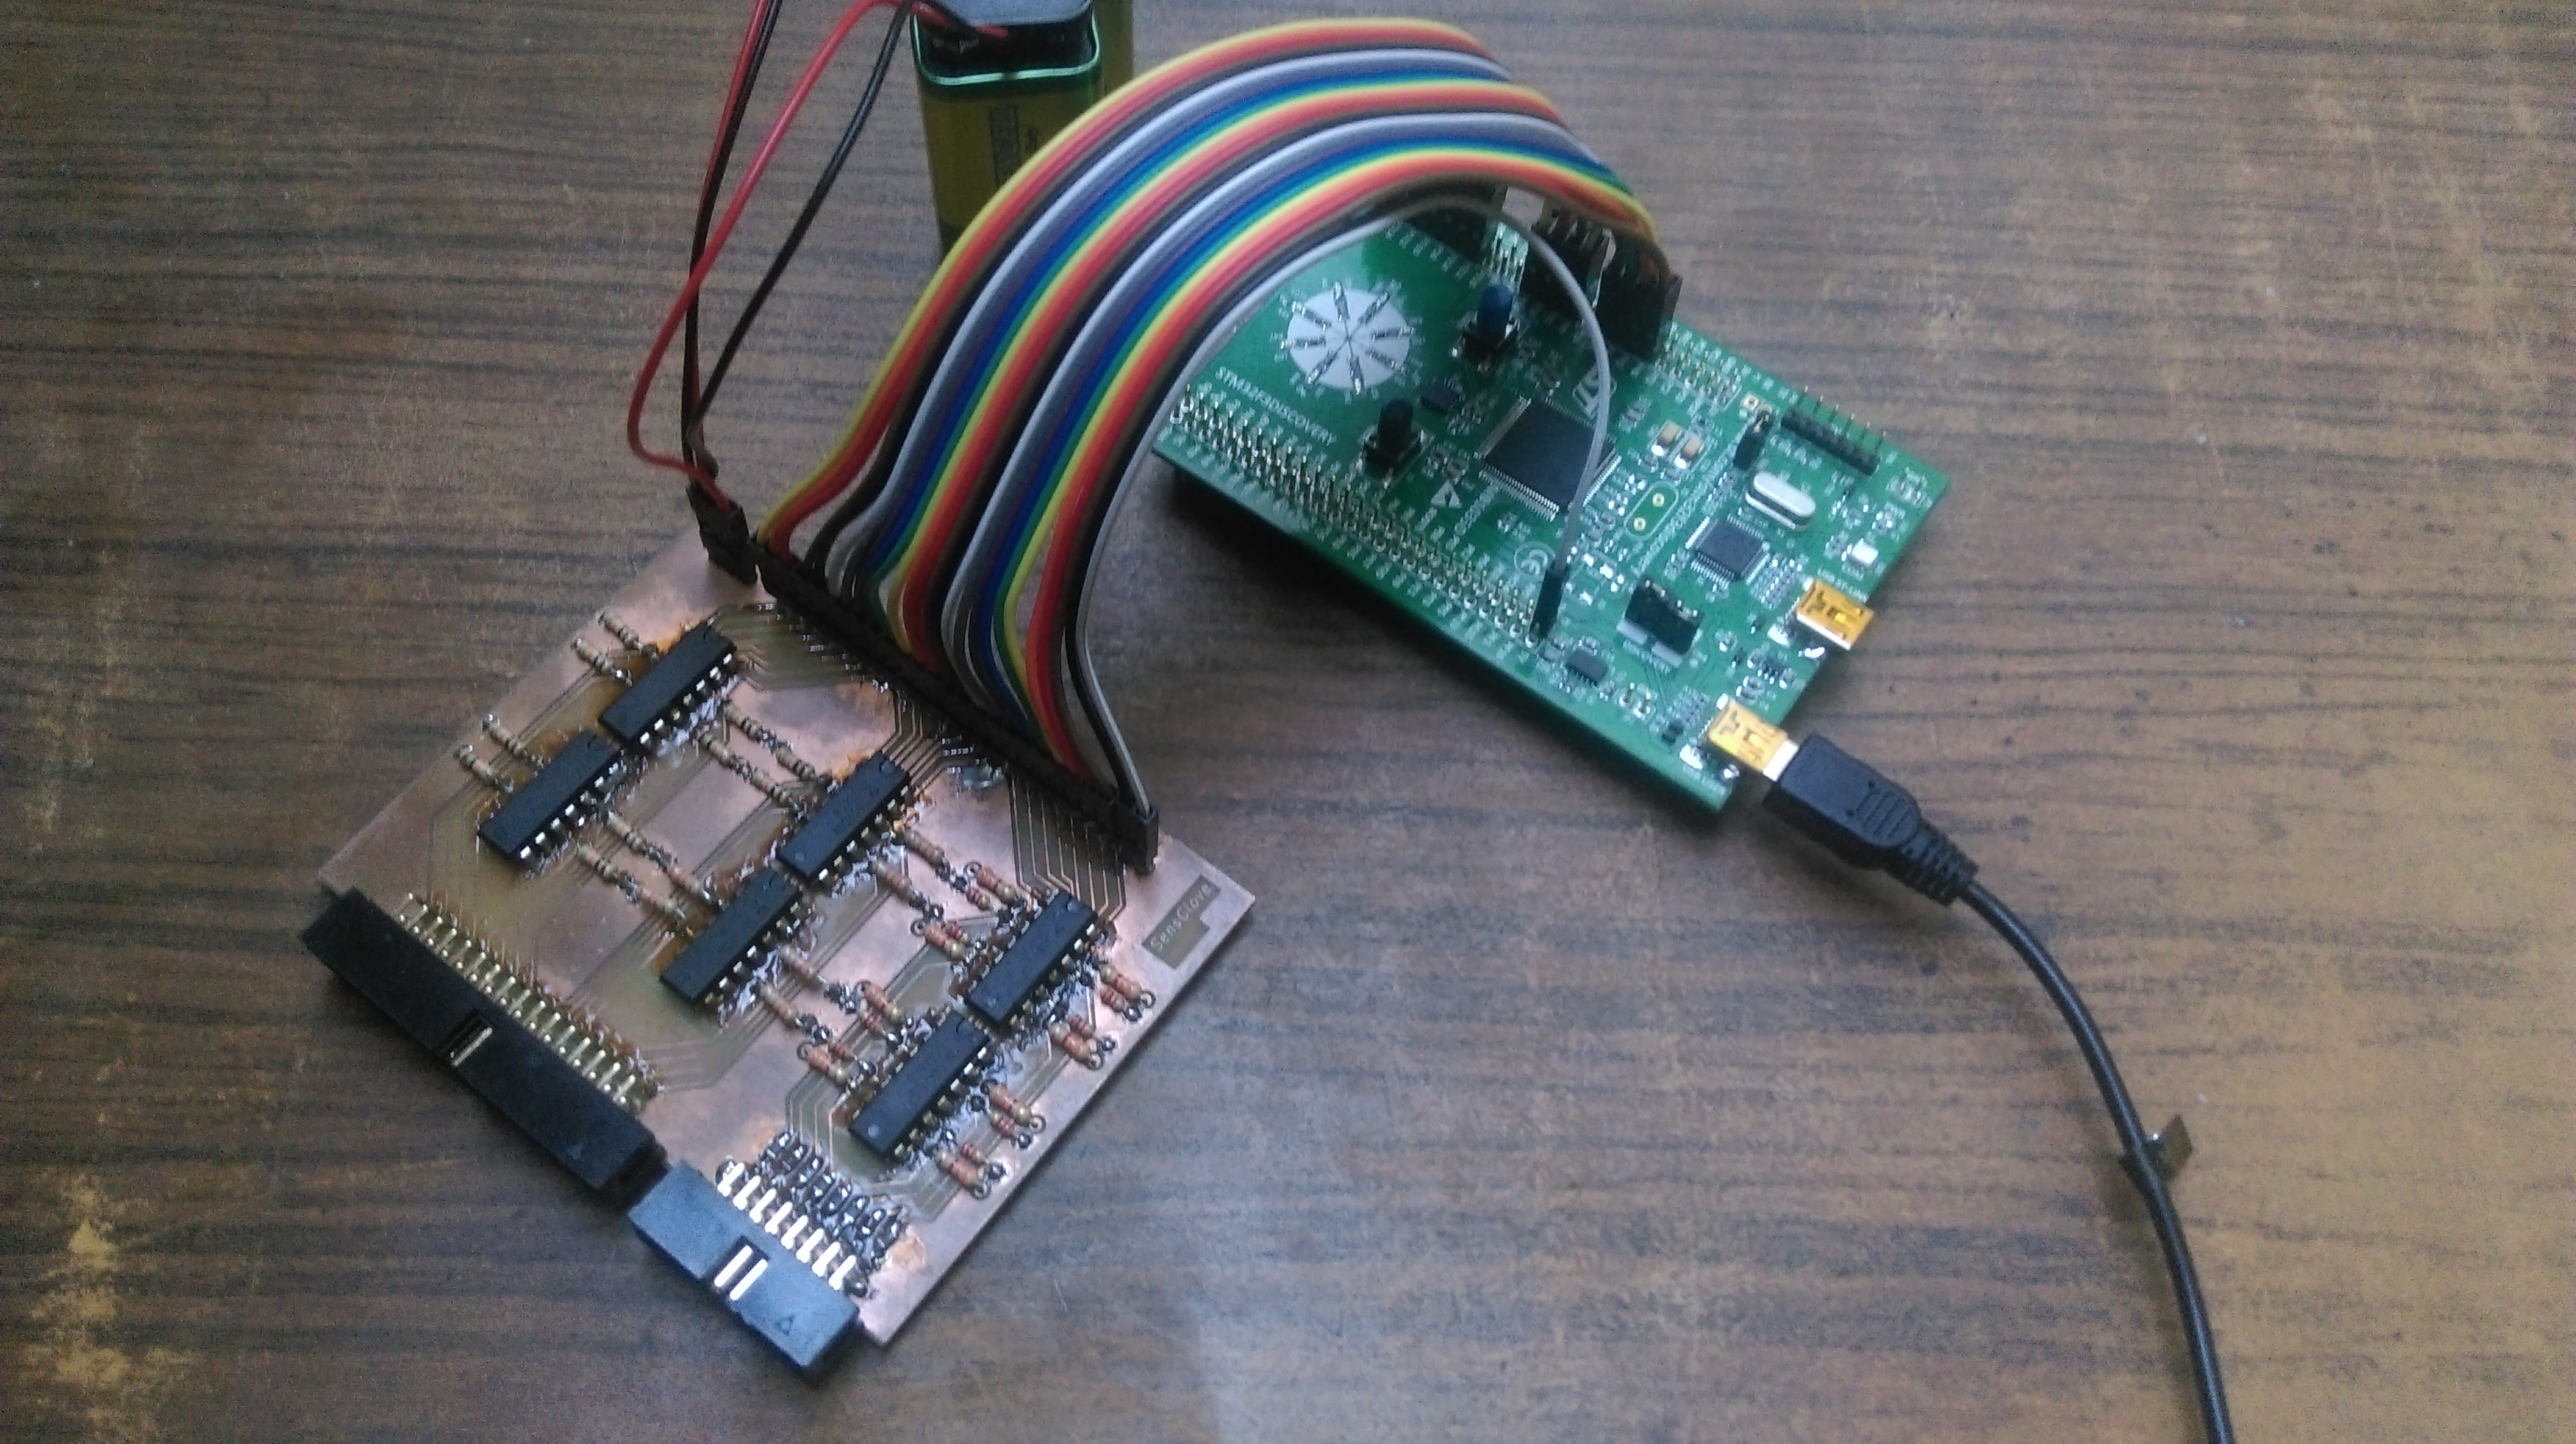
\includegraphics[width=10cm]{interfejs+discovery.jpg}
	\caption{Interfejs sprzętowy}
	\label{rys:interfejs_sprzetowy}
\end{figure}

\subsubsection{Schemat układu}

\begin{figure}[H]
	\centering
	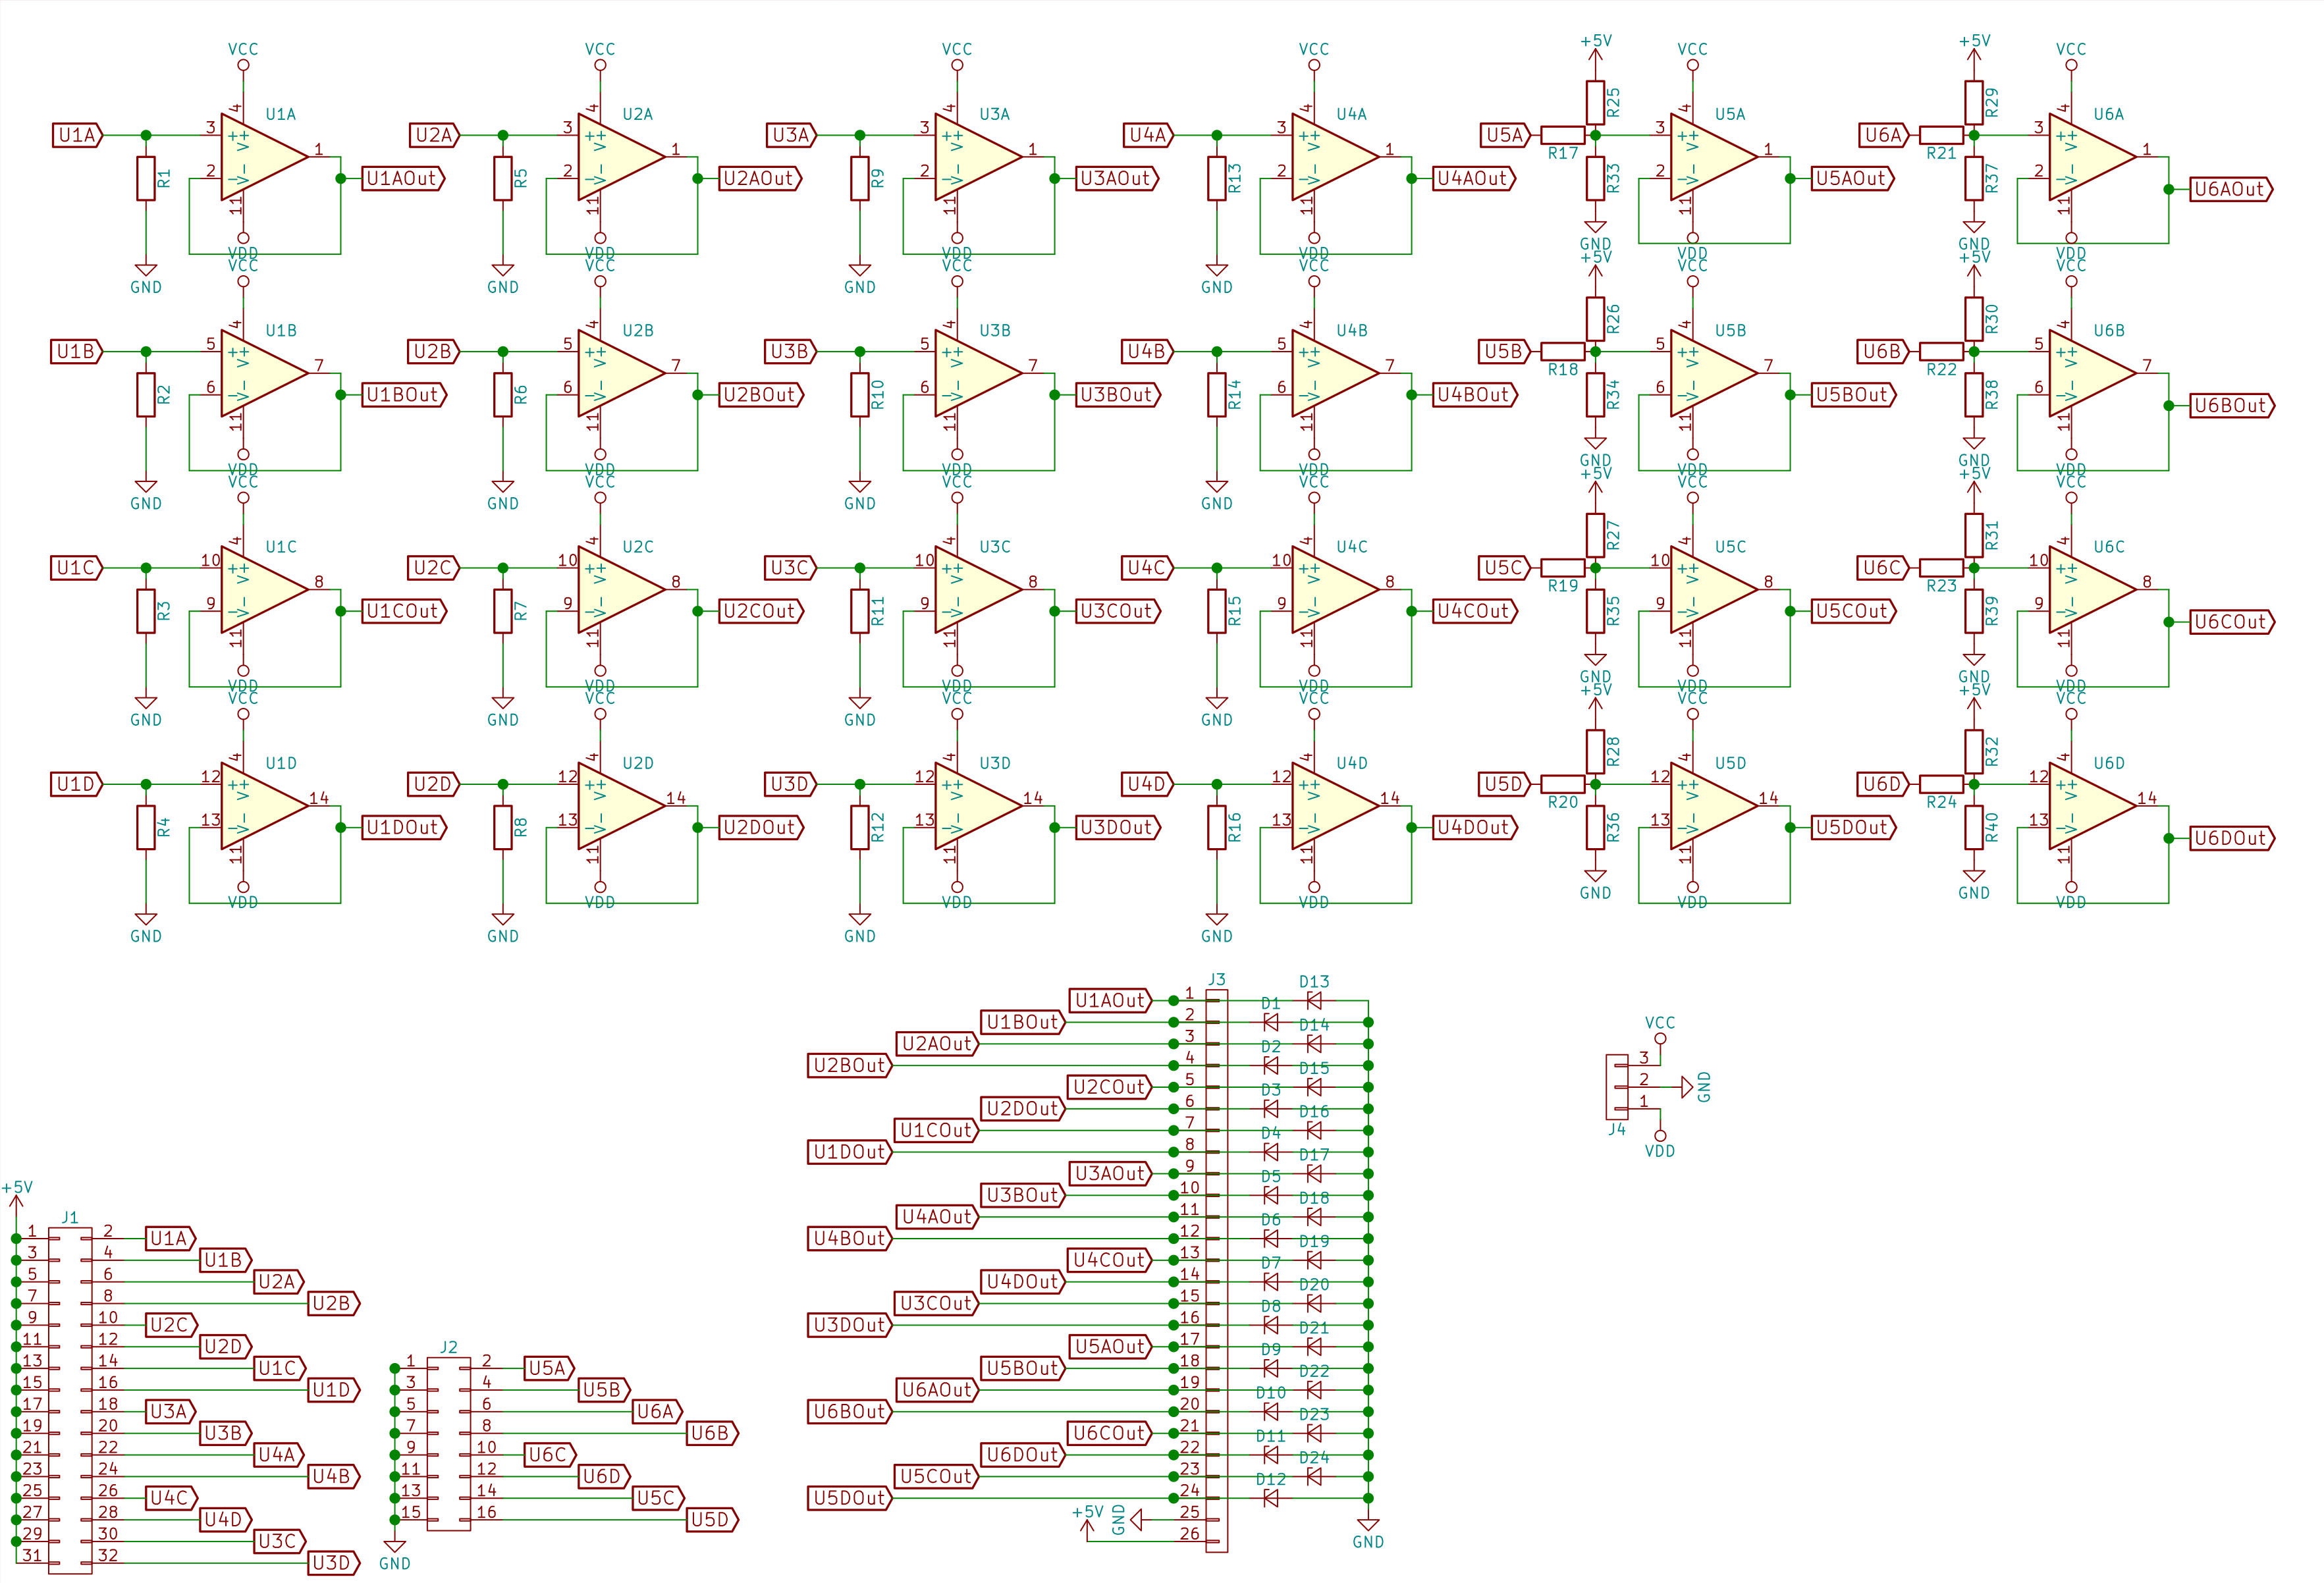
\includegraphics[width=14cm]{schemat.png}
	\caption{Schemat układu}
	\label{rys:schemat_ukladu}
\end{figure}

Projekt płytki pcb i wyprowadzenie pinów układu przedstawiono na rysunku  \ref{rys:pcb}.

\begin{figure}[H]
	\centering
	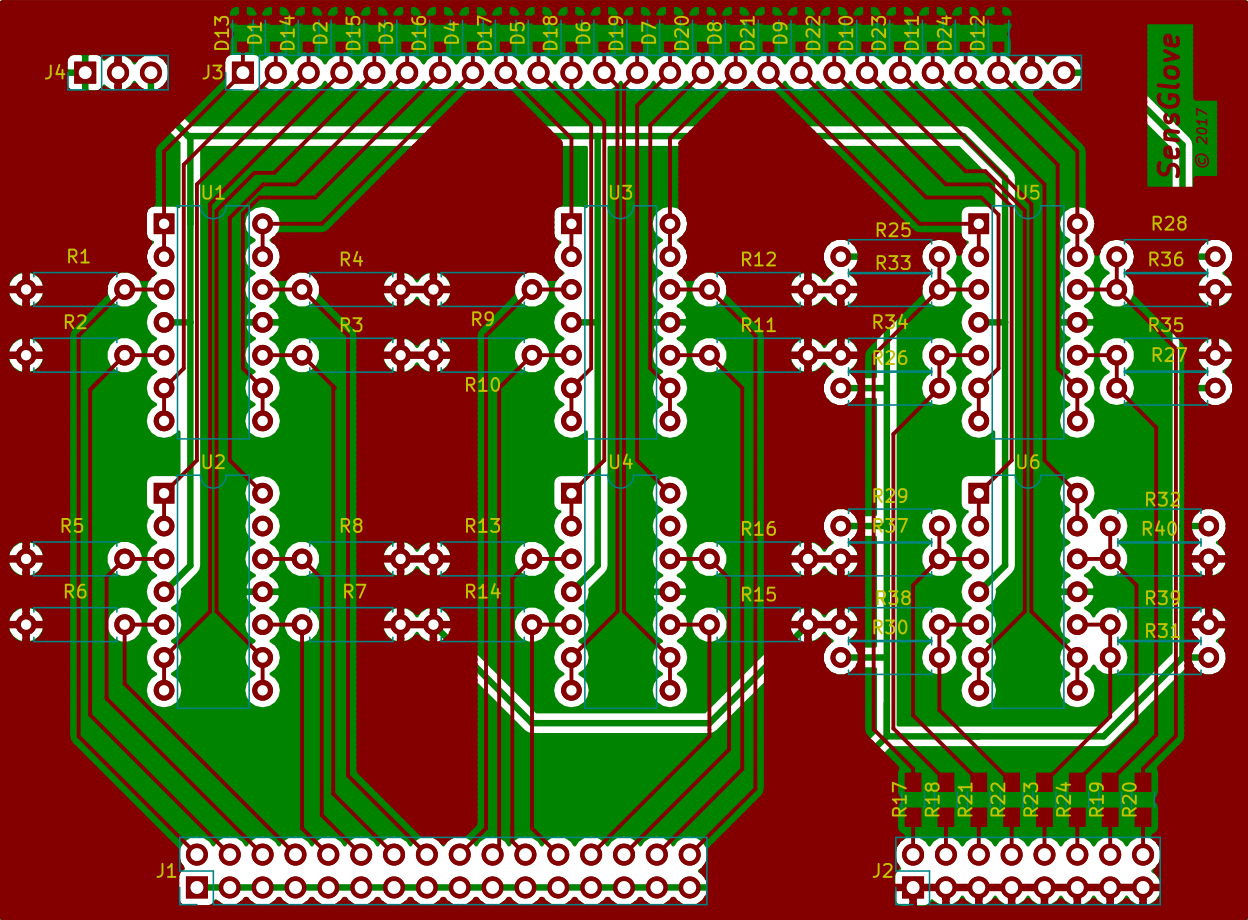
\includegraphics[width=12cm]{pcb.png}
	\caption{Schemat płytki pcb}
	\label{rys:pcb}
\end{figure}

\begin{figure}[H]
	\centering
	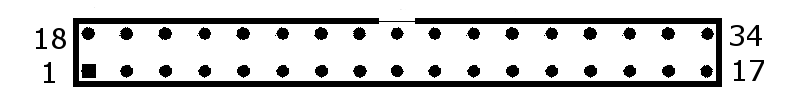
\includegraphics[width=9cm]{J1.png}
	\caption{J1 - pinout}
	\label{rys:J1 - pinout}
\end{figure}

\begin{table}[H]
	\centering
	\label{J1 - pinout}
	\begin{tabular}{ll}
	1 - 16		&	zasilanie czujników - +5v		\\
	17 - 27		&	złącza czujników nacisku 1 - 10		\\
	28 - 33		&	złącza czujników ugięcia 1 - 6		\\
	2, 34		&	NC					\\
\end{tabular}
\end{table}

\begin{figure}[H]
	\centering
	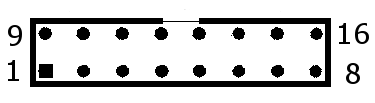
\includegraphics[width=6cm]{J2.png}
	\caption{J2 - pinout}
	\label{rys:J2 - pinout}
\end{figure}

\begin{table}[H]
	\centering
	\label{J2 - pinout}
	\begin{tabular}{ll}
	1 - 7		&	GND					\\
	8 - 16		&	złącza czujników biosygnałów 1 - 8	\\
\end{tabular}
\end{table}

\begin{figure}[H]
	\centering
	
\includegraphics[width=9cm]{J3.png}
	\caption{J3 - pinout}
	\label{rys:J3 - pinout}
\end{figure}

\begin{table}[H]
	\centering
	\label{J3 - pinout}
	\begin{tabular}{ll}
	1 - 10		&	sygnał czujników nacisku 1 - 10		\\
	11 - 16		&	sygnał czujników ugięcia 1 - 6		\\
	17 - 24		&	sygnał czujników biosygnałów 1 - 8	\\
	25		&	+5V					\\
	26		&	GND					\\
\end{tabular}
\end{table}

\begin{figure}[H]
	\centering
	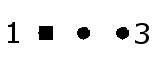
\includegraphics[width=6cm]{J4.png}
	\caption{J4 - pinout}
	\label{rys:J4 - pinout}
\end{figure}

\begin{table}[H]
	\centering
	\label{J4 - pinout}
	\begin{tabular}{ll}
	1 		&	-9V					\\
	2		&	GND					\\
	3		&	+9V					\\
\end{tabular}
\end{table}

\subsubsection{Połączenie z płytką STM32F3Discovery}
\begin{table}[H]
	\centering
	\label{Bill of materials}
\begin{tabular}{ll}
J1		&	ST3M32Discovery	\\
1		&	PB12		\\
2		&	PB14		\\
3		&	PB15		\\
4		&	PD8		\\
5		&	PD9		\\
6		&	PD10		\\
7		&	PD11		\\
8		&	PD12		\\
9		&	PD13		\\
10		&	PD14		\\

11		&	PB0		\\
12		&	PB1		\\
13		&	PE7		\\
14		&	PE8		\\
15		&	PE9		\\
16		&	PE10		\\

17		&	PA0		\\
18		&	PA3		\\
19		&	PA2		\\
20		&	PF4		\\
21		&	PA4		\\
22		&	PA5		\\
23		&	PA6		\\
24		&	PA7		\\

25		&	GND		\\
26		&	5V		\\
\end{tabular}
\end{table}

\subsubsection{Lista elementów}
\begin{table}[H]
	\centering
	\label{Bill of materials}
\begin{tabular}{lll}
U1-U6		&	TLC084CN			&	THT	\\
R1-R10		&	10kOhm				&	THT	\\
R11-R16		&	33kOhm				&	THT	\\
R17-R24		&	3.3kOhm				&	SMD	\\
R25-R32		&	3.3kOhm				&	THT	\\
R33-R40		&	2.2kOhm				&	THT	\\
D1-D24		&	3.3V Zenera			&	SMD	\\
J1		&	IDC-34 żeńskie			&	THT	\\
J2		&	IDC-16 żeńskie			&	THT	\\
J3		&	listwa kołkowa 1x26 2.56mm	&	THT	\\
J4		&	listwa kołkowa 1x3 2.56mm	&	THT	\\
\end{tabular}
\end{table}



\subsection{Kod programu}
\begin{verbatim}
//struktura danych do zapisu odczytu sygnałów
typedef union {
	struct {
		uint16_t forceSensors[10];
		uint16_t flexSensors[6];
		uint16_t biosignals[8];
		uint16_t checksum;
	}measure;
	uint16_t measures[25];
} data_t;
data_t data;

...

//konfiguracja DMA
  HAL_ADC_Start_DMA(&hadc1, &data.measure.biosignals[0], 4);
  HAL_ADC_Start_DMA(&hadc2, &data.measure.biosignals[4], 4);
  HAL_ADC_Start_DMA(&hadc3, &data.measure.flexSensors[0], 6);
  HAL_ADC_Start_DMA(&hadc4, &data.measure.forceSensors[0], 10);

...

//główna pętla programu
if(htim6_flag)
{
  data.measure.checksum = 0;
  for(int i = 0; i < 24; i++)
  {
    data.measure.checksum+=data.measures[i];
  }
  printf("X%4.4x%4.4x%4.4x%4.4x%4.4x%4.4x%4.4x%4.4x%4.4x%4.4x%4.4x%4.4x%4.4x%4.4x%4.4x%4.4x%4.
  4x%4.4x%4.4x%4.4x%4.4x%4.4x%4.4x%4.4x%4.4x\r\n",
	  data.measures[0], data.measures[1], data.measures[2], data.measures[3], data.measures[4],
	  data.measures[5], data.measures[6], data.measures[7], data.measures[8], data.measures[9],
	  data.measures[10], data.measures[11], data.measures[12], data.measures[13], data.measures[14],
	  data.measures[15], data.measures[16], data.measures[17], data.measures[18], data.measures[19],
	  data.measures[20], data.measures[21], data.measures[22], data.measures[23], data.measures[24]);
}
\end{verbatim}

%%%%%%%%%%%%%%%%%%%%%%%%%
\subsection{Program do akwizycji danych}

Osoby przedzielone do zadania: Ada Weiss, Małgorzata Witka-Jeżewska
\subsection{Opis klas programu}
Dokładny opis klas i poszczególnych parametrów tworzony jest za pomocą programu Doxygen.
\begin{figure}[H]
    \centering
    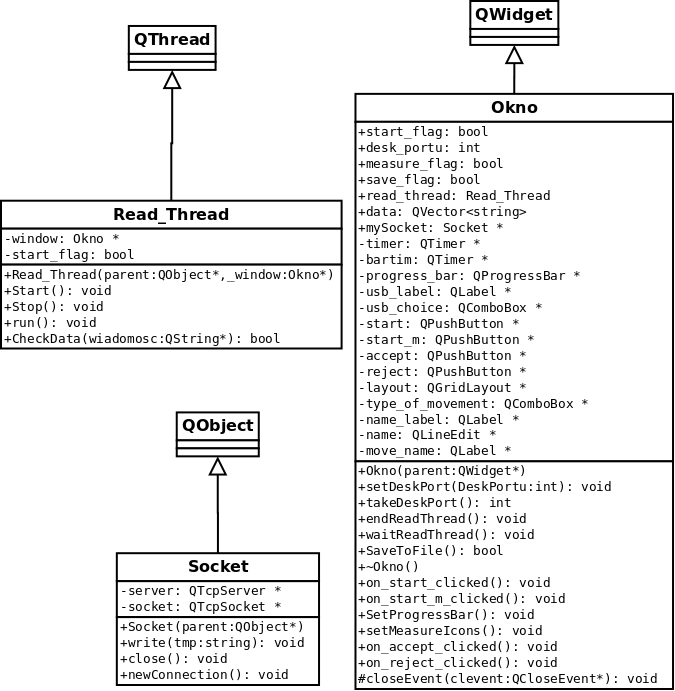
\includegraphics[scale=0.4]{autodia.png}
    \caption{Diagram klas programu}
    \label{rys:autodia}
\end{figure}

\begin{figure}[H]
    \centering
    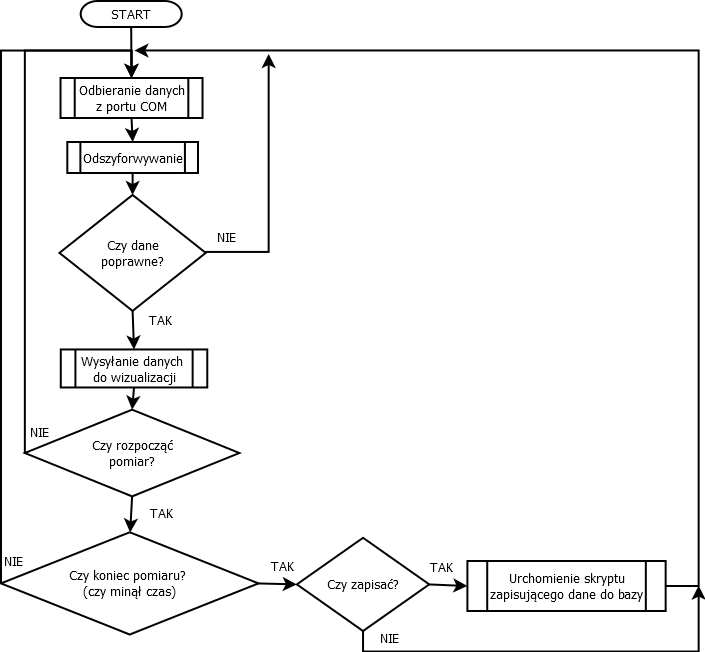
\includegraphics[scale=0.6]{programdia.png}
    \caption{Schemat ideowy działania programu}
    \label{rys:programdia}
\end{figure}

\subsubsection{Opis działania programu}

Interfejs graficzny programu został napisany z wykorzystaniem klas biblioteki Qt5 i został zaprezentowany na rys. \ref{rys:okno}. 
\begin{figure}[H]
    \centering
    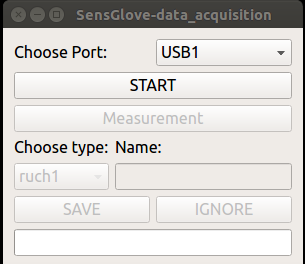
\includegraphics[scale=0.5]{okno.png}
    \caption{Okno główne programu}
    \label{rys:okno}
\end{figure}

Zasada działania została przedstawiona na rys. \ref{rys:programdia}. 
Pierwszym krokiem jest wybór portu USB i wciśnięcie przycisku start, co uruchamia konfiguracje wybranego portu USB. W przypadku braku podłączonego urządzenia na danym porcie wyświetlany jest komunikat przedstawiony na rys. \ref{rys:oknousb}. Kliknięcie ''Yes'' umożliwia ponowny wybór, a ''No'' kończy pracę programu.\\
\begin{figure}[H]
    \begin{center}
    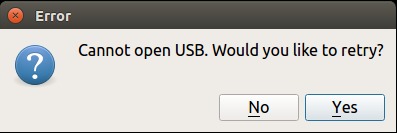
\includegraphics[scale=0.6]{oknousb.png}
    \caption{Komunikat o błędnym otwarciu USB.}
    \label{rys:oknousb}
    \end{center}
\end{figure}
Dane są odczytywane z poru USB w oddzielnym wątku Read\_thread, dziedziczącego po QThread. Zapewnia to odpowiednio szybką pracę programu. W tym samym wątku sprawdzana jest poprawność otrzymanej wiadomości (obliczanie sumy kontrolnej, sprawdzanie dlugości ciągu znaków) oraz wysyłanie danych do Socketu, który również został zaprogramowany z wykorzystaniem bibliotek Qt5 (klasa Socket).

W przypadku aktywowania przycisku ''Measurment'' aktywowany jest timer (na 2s) i dane te są zapisywane w wektorze 2000x23, z którego to jest możliwość zapisu danych do pliku w przypadku akceptacji pomiaru po jego ukończeniu. Widok okna w trakcie pomiaru przedstawia \ref{rys:oknopomiar}.
\begin{figure}[H]
    \centering
    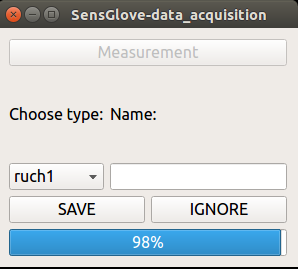
\includegraphics[scale=0.6]{oknopomiar.png}
    \caption{Okno główne programu w trakcie pomiaru}
    \label{rys:oknopomiar}
\end{figure}

Akceptacja pomiaru wymaga również podania imienia użytkownika oraz wyboru ruchu który jest wykonywany. Program wywołuje po zapisie do pliku skrypt który umieszcza plik w bazie danych.

Można również dany pomiar zignorować, np. w przypadku stwierdzenia, że został on błędnie wykonany.

\subsubsection{Format danych}
Ramka danych:
\begin{itemize}
    \item znak X,
    \item 23 sygnały z czujników w postaci 4 znaków w systemie szesnastkowym,
    \item suma kontrolna w postaci dwóch znaków w systemie szesnastkowym,
    \item znak końca linii \textbackslash r \textbackslash n;
\end{itemize}

%%%%%%%%%%%%%%%%%%%%%%%%%
\subsection{Baza danych}
Osoby przydzielone do zadania: Beata Berajter, Dorota Gidel.

\subsubsection{Wprowadzone zmiany}
Zdecydowano się na zmianę struktury bazy danych. Zamiast umieszczania trzech osobnych plików zawierających dane odpowiednio z czujników nacisku, zgięcia i elektrod, tworzony będzie tylko jeden plik zawierający wszystkie te dane w takiej kolejności. Plik taki zawierać będzie 2000 linii i 23 kolumny odczytów. Dodatkowo, nazwa pliku nie będzie zawierać daty gdyż można ją uzyskać z daty tworzenia pliku. Nowy schemat struktury bazy danych przedstawiono na rysunku \ref{rys:baza_danych}.
\begin{figure}[H]
    \centering
    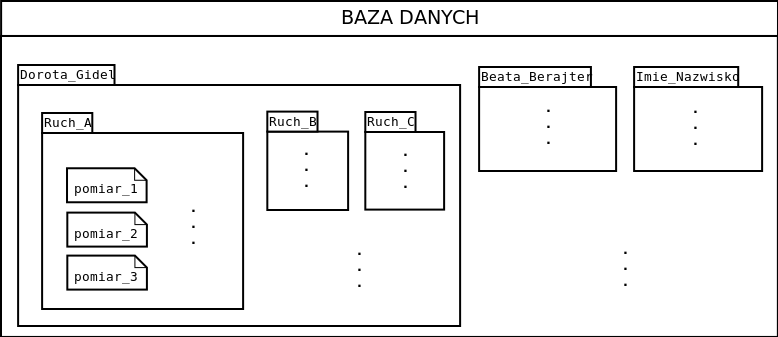
\includegraphics[width=\textwidth]{baza_danych.png}
    \caption{Schemat struktury bazy danych}
    \label{rys:baza_danych}
\end{figure}

\subsubsection{Opis działania skryptu}
Stworzony skrypt do umieszczania w odpowiednim miejscu plików z odczytami napisany jest w powłoce bash. Przykładowe wywołanie skryptu wgląda następująco:\\

\texttt{\$ bash przeniesPlik sciezka/do/pliku/z/danymi Imie NazwaRuchu}\\ \\
Skrypt przenosi podany plik (\texttt{sciezka/do/plik/z/danymi}) do głownego folderu bazy danych który zdefiniowany jest jako katalog o nazwie ''baza\_danych'' w katalogu domowym. Dzięki podanym argumentom umieszcza plik w odpowiednim miejscu. Numeracja pliku po kolei jest zapewniona przez prowadzenie spisu w osobnym pliku tekstowym należącym do bazy danych. Dla bezpieczeństwa sprawdzane jest też czy w wywołaniu skryptu została podana wystarczająca liczba argumentów.

%%%%%%%%%%%%%%%%%%%%%%%%%
\subsection{Wizualizacja danych}
Osoby przydzielone do zadania: Dorota Gidel, Katarzyna Wądrzyk.

\subsubsection{Ogólny diagram klas}
Na rysunku \ref{rys:diagram_ogolny} zaprezentowano ogólny diagram klas w programie wizualizującym dane z czujników.
\begin{figure}[H]
    \centering
    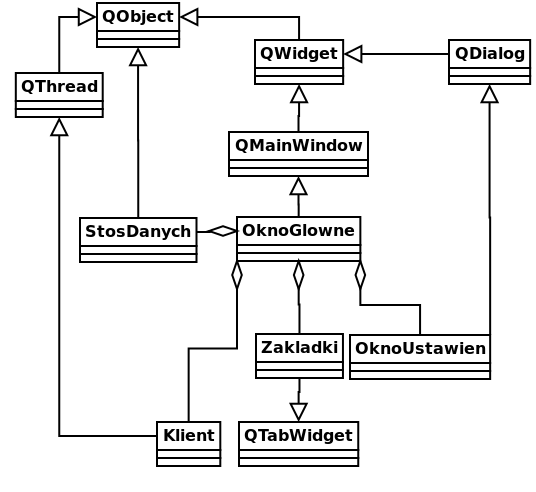
\includegraphics[width=11cm]{diagram_ogolny.png}
    \caption{Ogólny diagram klas - wizualizacja}
    \label{rys:diagram_ogolny}
\end{figure}

\subsubsection{Diagram klas zakładek}
Na obrazku \ref{rys:diagram_klas} zaprezentowano ogólny diagram klas zakładek zawierających wykresy i prezentacje odpowiednio z czujników nacisku oraz zgięcia.
\begin{figure}[H]
    \centering
    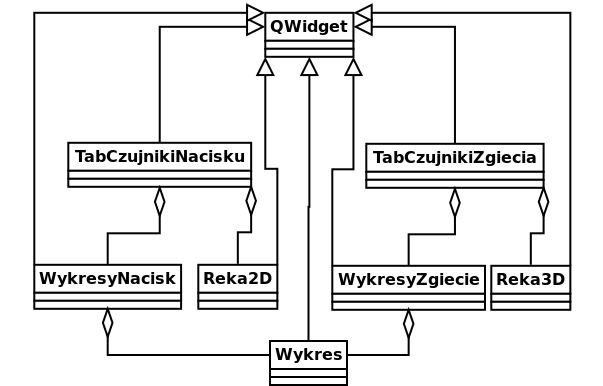
\includegraphics[width=11cm]{diagram_klas.png}
    \caption{Diagram klas zakładek - wizualizacja}
    \label{rys:diagram_klas}
\end{figure}

\subsubsection{Interfejs użytkownika}
Aplikacja automatycznie próbuje się połączyć z portem 2666 na localhostcie. Jeżeli użytkownik chce skorzystać z innego portu lub nazwy/ip serwera może wprowadzić zmiany w ustawieniach. Dostęp do ustwień jest z górnego paska po lewej stronie. Isnieje dodatkowo możliwość zmiany zakresu czasu prezentaowanego na wykesach. Domyślnie wartość ta wynosi 30 s.\\
W trakcie odbierania danych istnieje możliwość zatrzymania wykresów i wizualizacji dłoni w danym momencie poprzez przyciśnięcie przycisku ''Stop''. \\
Rysunek \ref{rys:zakladka1} przedstawia pierwszą zakładkę aplikacji wizualizującej dane - czujniki nacisku. Po lewej stronie umieszczone są wykresy. Pierwszy największy wykres, można zmieniać przyciskając odpowiednio wykres który chcemy najbardziej śledzić. Wybrany wykres zaznaczony jest przez kolorową obwódkę. Po prawej stronie znajduje się widget zawierający ręke 2D prezentującą przez kolory odczytywane w danym momencie wartości napięcia.
\begin{figure}[H]
    \centering
    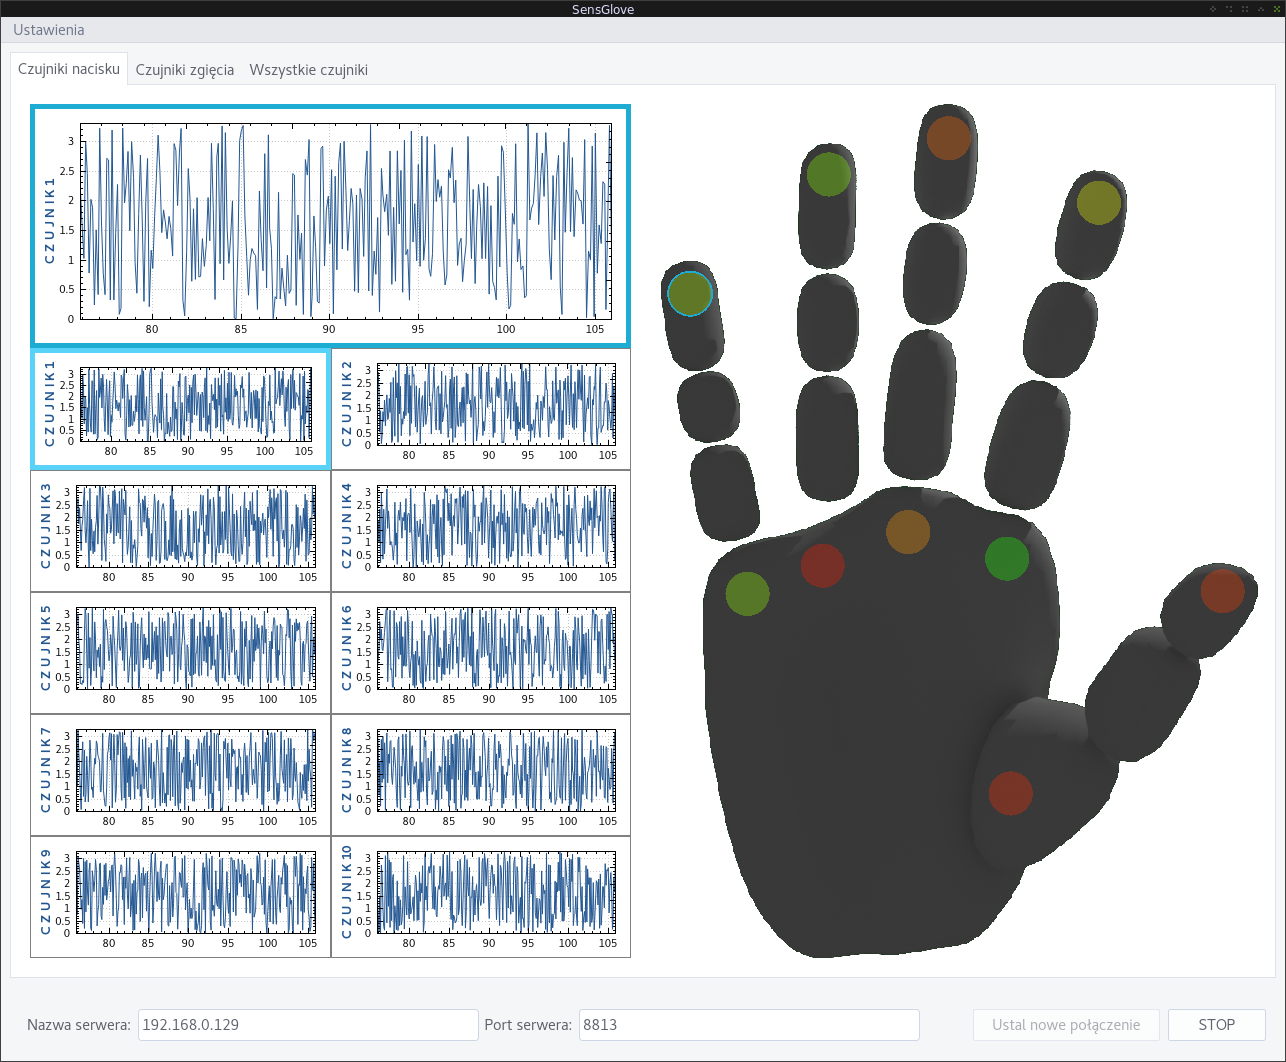
\includegraphics[width=16cm]{zakladka1.png}
    \caption{Zakładka 1}
    \label{rys:zakladka1}
\end{figure}
Rysunek \ref{rys:zakladka2} przedstawia drugą zakładkę aplikacji wizualizującej dane - czujniki zgięcia. Po lewej stronie tak samo jak poprzednio znajdują się wykresy odczytywanego napięcia. Po prawej stronie znajduje się widget zawierający ręke 3D której palce zginają się odpowiednio do otrzymywanych wartości z czujników.
\begin{figure}[H]
    \centering
    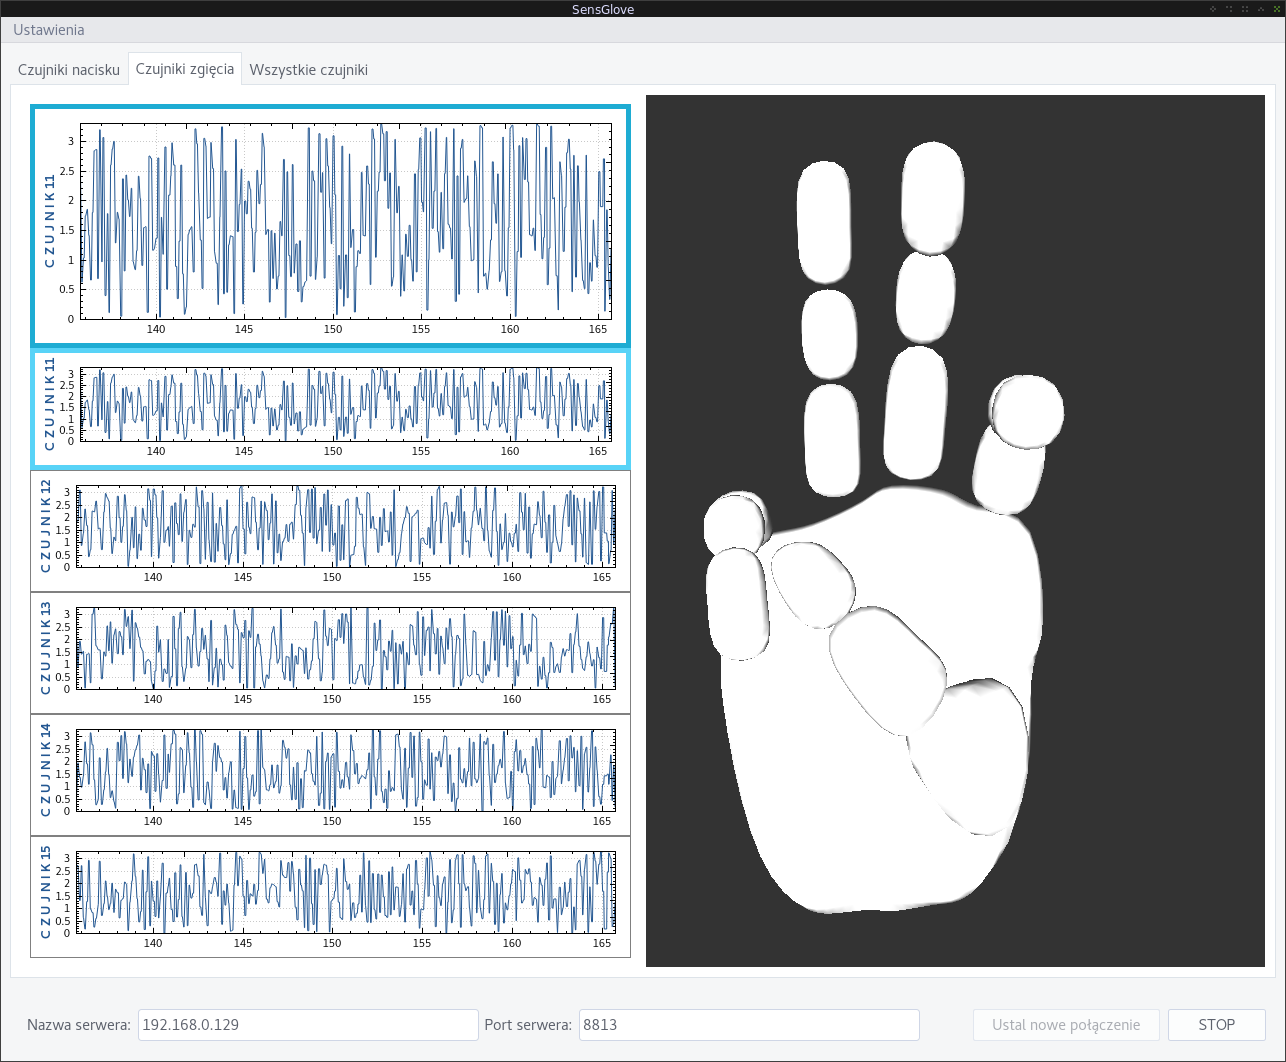
\includegraphics[width=16cm, height=10cm]{zakladka2.png}
    \caption{Zakładka 2}
    \label{rys:zakladka2}
\end{figure}
Rysunek \ref{rys:zakladka3} przedstawia trzecią zakładkę prezentującą odczyty EMG biosygnałów z elektrod w formie wykresów.
\begin{figure}[H]
    \centering
    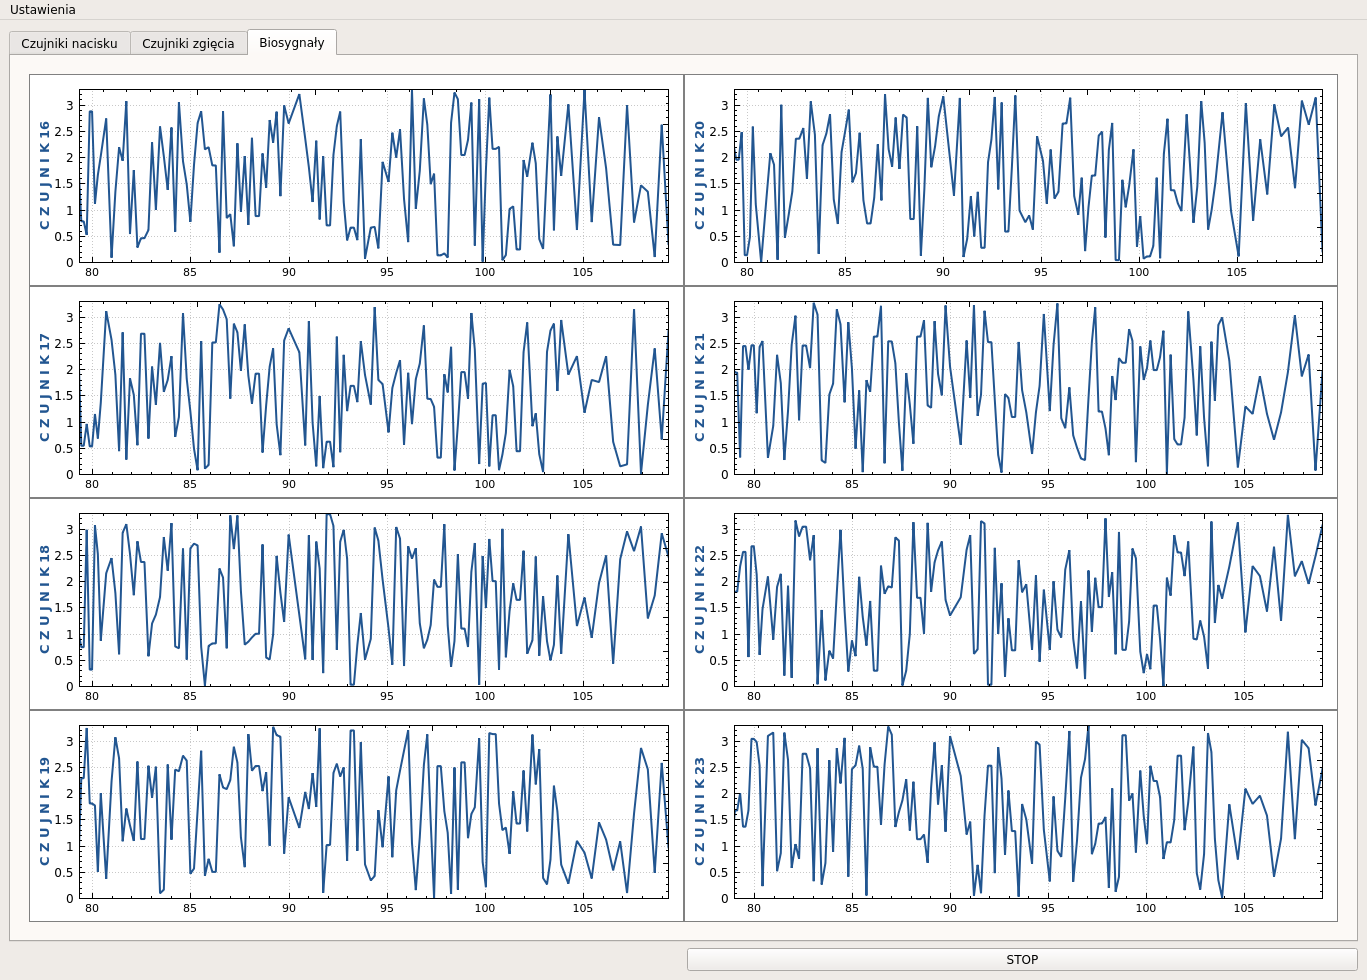
\includegraphics[width=16cm, height=9.5cm]{zakladka3.png}
    \caption{Zakładka 3}
    \label{rys:zakladka3}
\end{figure}


Aplikacja odbiera pomyślnie dane z programu do akwizycji oraz wizualizuje zinterpretowane pomiary na wykresach i modelach dłoni. 


\section{Testowanie całości systemu i rozpowszechnianie}
Po połączeniu wszytkich komponentów projektu przeprowadzono testy. Polegały one na wykonywaniu ruchów w rękawiczce sensorycznej i obserwowanie efektów w programie wizualizującym oraz sprawdzenie poprawnego zapisu pliku do bazy danych. Testy pokazały, że sygnały przeysłane są odbierane poprawnie, co pokazują zdjęcia i film umieszczony na stronie internetowej  \url{http://sensglove.happyrobotics.com} w odpowiednich zakładkach. Na stronie został również zamieszczony link do strony GitHub \url{https://github.com/Sensglove/SG}, na której zamieszczony jest kod oprogramowania i dokumentacja.

\section{Podsumwoanie}
Projek spełnia początkowe założenia. Rękawiczka jak i okablowanie do niej nie krępują ruchu, płytka wzmacnia i przesyła pomiary z 22 czujników z możliwością dołączenia dwóch kolejnych. Program do akwizycji w czasie rzeczywistym pobiera dane ze wszystkich sensorów z możliwością zapisu danych do konkretnych katalogów oraz przekazuje do programu wizualizującego, który w czasie zbliżonym do rzeczywistego przedstawia reakcje czujników na ruch.

\end{document}
